\documentclass{article}
    \usepackage[utf8]{inputenc}
    \usepackage[T2A]{fontenc}
    \usepackage[english,russian]{babel}

    % Related to math
    \usepackage{amsmath,amssymb,amsfonts,amsthm}

    \usepackage{graphicx}
    \graphicspath{{media/}}

    \usepackage{multicol}

\begin{document}

\section{Моделирование маршрута инструмента для машин фигурной листовой резки с ЧПУ. Основные понятия и задачи}

\subsection{Технологии и техники листовой резки на машинах с ЧПУ}

В машиностроении, в производстве металлоконструкций
и в других отраслях промышленности существенная часть продукции
зготавливается из заготовок,
получаемых из листовых материалов на различном технологическом оборудовании.
К такому оборудованию относятся, в частности,
Используемые на предприятиях отечественные и зарубежные
системы автоматизированного проектирования (САПР),
предназначенные для разработки управляющих программ (УП)
для машин листовой резки с ЧПУ (т.н. Computer-Aided Manufacturing, CAM-системы)
обеспечивают автоматизацию процесса разработки УП,
однако не позволяют решить многие оптимизационные задачи.
При этом при моделировании маршрута инструмента пользователям
САПР часто приходится применять интерактивные методы проектирования УП,
поскольку алгоритмы генерации УП,
реализованные в автоматическом режиме проектирования,
во многих случаях не позволяет генерировать оптимальные управляющие программы,
а также обеспечить соблюдение некоторых технологических требований листовой резки.
В качестве критериев оптимизации имеются в виду время резки и
некоторые другие стоимостные характеристики процесса листовой резки.
Проблема разработки методов, алгоритмов и соответствующего программного обеспечения,
позволяющих в автоматическом режиме оптимизировать параметры
процесса резки заготовок из листовых материалов на машинах с числовым программным управлением,
включая алгоритмы маршрутизации движения инструмента,
которые бы обеспечивали минимизацию времени резки и стоимости процесса,
остается актуальнейшей задачей раскройно-заготовительного производства.

Рассмотрим понятие маршрута инструмента (маршрута резки)
применительно к некоторым технологиям фигурной листовой резки.
В настоящее время в промышленном производстве
единичного и мелкосерийного типа для раскроя листовых материалов
используются в основном следующие технологии:
лазерная, плазменная, газовая и гидроабразивная.
Целесообразность их применения определяется различными технологическими факторами,
например, свойствами раскраиваемого материала,
экономическими требованиями к процессу резки,
требованиями к качеству реза и пр.
Эти и некоторые другие технологии резки предполагают,
что для сохранения требуемой геометрии заготовки
траектория движения режущего инструмента не совпадает
с граничным контуром заготовки,
а задается некоторой эквидистантой этого контура,
поскольку часть материала вырезается («сгорает», «вымывается» и пр.)
в процессе резки.
Как правило, дистанция между эквидистантным контуром,
по которому осуществляется резка, и граничным контуром заготовки определяется величиной,
равной половине ширины реза.
Эта величина зависит от выбранной технологии резки,
толщины и марки материала, заданной скорости резки
и особенностей конкретного технологического оборудования,
используемого для резки.

Еще она особенность листовой резки –
необходимость предварительной врезки (пробивки)
материала перед процессом резки непосредственно
по эквидистантному контуру заготовки.
Пробивка материала сопровождается дополнительными
деформациями материала в точке врезки,
поэтому производится на расстоянии (дистанции)
от контура заготовки большем,
чем дистанция до эквидистантного контура за исключением случаев,
когда для точек врезки в листовом материале механическим способом
готовятся (например, просверливаются)
отверстия.
Врезка может также осуществляться
непосредственно на границе материала
(«врезка с края листа»).
В этом случае достигается уменьшение
деформаций материала и сокращается время врезки.

Один из способов резки заготовки (стандартная техника)
показан на Рис. \ref{standard-cutting}.

\begin{figure}
  \begin{center}
  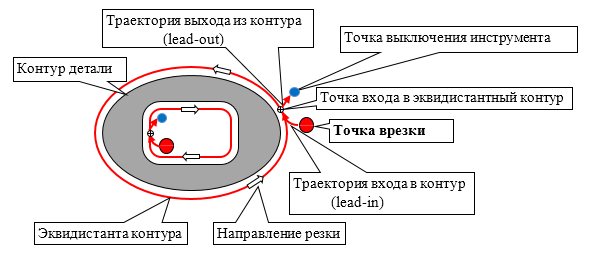
\includegraphics[width=0.9\textwidth]{cutting-path.png}
  \caption{Схема стандартной техники резки (резка по замкнутому контуру)}
  \label{standard-cutting}
  \end{center}
\end{figure}

Если используется стандартная техника резки,
то в этом случае каждый замкнутый контур вырезается целиком,
и после резки одного контура переход к следующей точке врезки
происходит с выключенным инструментом на холостом ходе.
При этом точка выключения инструмента, в общем случае,
может не совпадать с точкой входа в эквидистантный контур заготовки,
по которому осуществляется резка, и также как и точка врезки
может лежать вне заданного эквидистантного контура.
Во многих случаях допускается программирование точки выключения
инструмента непосредственно на эквидистантном контуре.

Стратегия минимизации тепловых деформаций при термической резке
и требования к качеству реза порождают необходимость управления
не только выбором точек врезки,
но и управлением траекторией подхода к контуру (lead-in)
и способом выхода из контура (lead-out).
В зависимости от конкретных условий
(вида термической резки, марки и толщины материала,
скорости резки, геометрической формы контура и пр.)
подход к контуру может осуществляться по дуге окружности,
касательная к которой совпадает с касательной к контуру в точке входа,
либо производиться по прямой линии
(например, по наикратчайшему расстоянию до контура).
Соответственно и после завершения резки выход из контура
также может осуществляться с включенным инструментом
(либо по дуге, либо по прямой линии).
Необходимость выхода из контура с включенным
инструментом может быть вызвана тем,
что в точке выключения инструмента может возникнуть
«вырыв» или оплавление части материала,
что приводит к искажению геометрии заготовки.
Уменьшение эффекта деформации заготовок обеспечивает
также врезка в «угловые» точки заготовок
(Рис. \ref{corner}).

\begin{figure}
  \begin{center}
  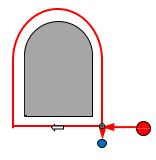
\includegraphics[width=0.3\textwidth]{corner.png}
  \caption{Пример врезки «в угол»}
  \label{corner}
  \end{center}
\end{figure}

Примером нестандартной техники
может служить «цепная» резка,
которая заключается в резке нескольких контуров с
использованием одной точки врезки.
При этом каждый контур,
как и в случае применения стандартной техники резки,
вырезается целиком.
На Рис. \ref{chain}
показан пример схемы резки двух заготовок,
в которой резка внешних контуров обеих заготовок
производится без выключения инструмента
с использованием только одной точки врезки.

\begin{figure}
  \begin{center}
  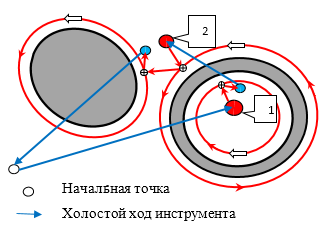
\includegraphics[width=0.5\textwidth]{chain.png}
  \caption{Пример схемы резки двух заготовок с использованием стандартной и «цепной» техники резки}
  \label{chain}
  \end{center}
\end{figure}

Перемещение инструмента в точку врезки
в этом примере начинается из начальной точки на холостом ходу,
а после завершения резки последнего контура
предусмотрен возврат инструмента в начальную точку.

На практике применяется также техника резки
замкнутого контура заготовок по частям
с использованием нескольких точек врезки
с целью формирования т.н. «перемычек»
(Рис. \ref{jumper}),
а также используются другие специальные приёмы,
целью которых является оптимизация различных параметров,
характеризующих процесс резки,
и соблюдение необходимых технологических требований резки.
Техника резки «перемычка» предусматривает
оставление не вырезанной части контура заготовки обычно,
небольшого прямолинейного отрезка или нескольких отрезков,
с резкой этих отрезков после завершения резки оставшейся части контура.
Этот прием применяется с целью уменьшения деформаций материала
при термической резке заготовок, склонных к термическим деформациям,
в частности, длинномерных заготовок.
На рис. \ref{saber} показан пример искажения геометрической формы
(получения т.н. формы «сабли»)
и изменения размера длинномерной прямоугольной заготовки,
вырезаемой без использования техники «перемычка»

\begin{figure}
  \begin{center}
  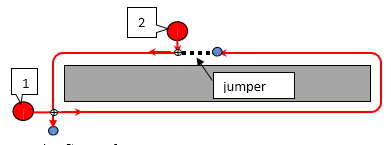
\includegraphics[width=0.5\textwidth]{jumper.png}
  \caption{Схема формирования перемычки на контуре при резке полосы}
  \label{jumper}
  \end{center}
\end{figure}

\begin{figure}
  \begin{center}
  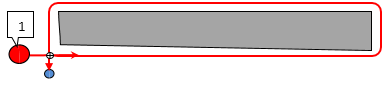
\includegraphics[width=0.5\textwidth]{saber.png}
  \caption{Результат изменнения формы и размера прямоугольной заготовки при термической резке}
  \label{saber}
  \end{center}
\end{figure}

На Рис. \ref{bridge}
приведен пример использования техники «мост»,
предполагающей  частичную резку замкнутого контура
заготовки с последующим завершением резки контура
после резки контура другой заготовки или
группы контуров других заготовок.
Эта техника используется при резке двух или
нескольких рядом расположенных заготовок и
предусматривает переход по короткой траектории («мосту»)
к резке другой заготовки и возврат к первому контуру
по этой же траектории для завершения процесса резки.
Так же, как и «перемычки»,
мосты существенно уменьшают тепловые деформации материала,
особенно при резке длинномерных заготовок,
кроме того, сокращают число точек врезки.

\begin{figure}
  \begin{center}
  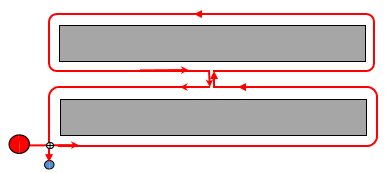
\includegraphics[width=0.5\textwidth]{bridge.png}
  \caption{Схема резки двух полос с использованием техники «мост»}
  \label{bridge}
  \end{center}
\end{figure}

Разновидностью техники мост можно считать технику змейка
(Рис. \ref{snake}),
в которой также используется прием
частичной резки контура и резку
нескольких заготовок без выключения инструмента.

\begin{figure}
  \begin{center}
  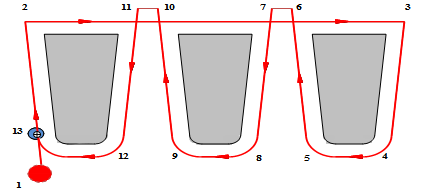
\includegraphics[width=0.7\textwidth]{snake.png}
  \caption{Схема резки «змейка»}
  \label{snake}
  \end{center}
\end{figure}

Для уменьшения длины рабочего хода инструмента
применяют т.н. «совмещенный» рез.
Он используется для вырезки заготовок,
которые содержат прямолинейные отрезки в контуре,
и которые в процессе раскроя размещаются таким образом,
что имеют общую границу по одному из таких прямолинейных отрезков.
Общая прямолинейная граница позволяет размещать
заготовки с половинным припуском на рез
(т.е., на ширину реза),
поскольку режется только один раз,
что экономит материал и сокращает суммарную
длину резки на величину совмещенного реза.
Совмещенный рез реализован, в частности,
в технике резки «восьмёрка»,
применяемой для резки двух одинаковых заготовок
(Рис. \ref{8}).
В этом технике используется также идея цепной резки.

\begin{figure}
  \begin{center}
  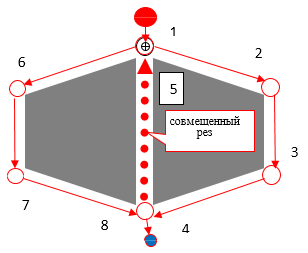
\includegraphics[width=0.6\textwidth]{8.png}
  \caption{Схема резки «восьмеркой» двух заготовок}
  \label{8}
  \end{center}
\end{figure}

Основные технологические требования
фигурной резки на машинах с ЧПУ обусловлены
необходимостью учёта возникающих деформаций
материала и искажения геометрических размеров
вырезаемых заготовок при использовании
термических технологий резки.
Применение специальных техник позволяет
уменьшить эффект искажения геометрии,
который особенно значителен при
использовании газовой и плазменной технологий.

При использовании любой техники резки маршрут инструмента
машины с ЧПУ для фигурной листовой резки
включает в себя следующие компоненты:
\begin{enumerate}
  \item точки врезки;
  \item рабочий ход инструмента;
  \item точки выключения инструмента;
  \item линейное перемещение инструмента на холостом ходе
  между точкой выключения инструмента и следующей точкой врезки.
\end{enumerate}

При разработке управляющей программы
первое перемещение инструмента обычно
программируется, как на Рис. \ref{chain},
из начальной точки.

Отметим, что некоторые машины фигурной листовой
резки с ЧПУ могут быть укомплектованы с
пециальным видом инструмента,
т.н. трехрезаковым блоком для вырезания
из листа заготовок с одновременной разделкой
кромок поверхности реза для последующей сварки.
Врезка в материал для такого инструмента
программируется специальными способами.
Вопросы применения трехрезакового блока
в рамках данной работы не рассматриваются.
Также мы не будем рассматривать вопросы
маршрутизации инструмента для машин
листовой резки с несколькими суппортами.

Введём некоторые определения,
касающиеся понятия маршрута резки.
В дальнейшем при формальном обозначении
математических и геометрических категорий
мы будем использовать стандартную
теоретико-множественную символику.
Ее детальное описание дано в 3.1.
%%% TODO! Fix reference ^^^^^^^^^^^^^^
Введем следующие определения.

{\bfСегментом резки}
$S=MM^*$
будем называть траекторию рабочего хода
инструмента между точкой врезки
$M$
и соответствующей ей точкой выключения инструмента
$M^*$.
Геометрически сегмент резки представляет собой
определенную на эвклидовой плоскости
$\mathbb R^2$
кривую.
$(S \subset \mathbb R \times \mathbb R;
M=(x,y) \in \mathbb R \times \mathbb R,
M^* =(x^*,y^*)\in \mathbb R \times \mathbb R)$
Будем также полагать,
что в каждой точке траектории определено направление движения инструмента.
Заметим, что если сегмент резки не содержит замкнутых контуров,
то направление движения резки в каждой точке траектории
однозначно определяется начальной точкой сегмента
(точкой врезки).
Замкнутые контуры в траектории рабочего хода инструмента
могут появляться не только в результате резки контуров заготовок,
но и при программировании т.н. петель,
которые используются для повышения качества реза.

Используя понятие сегмента резки,
все техники фигурной резки на машинах с ЧПУ
можно разделить на 3 класса:
\begin{enumerate}
  \item
  {\it Резка по замкнутому контуру (стандартная техника)}:
  в этом случае сегмент резки содержит
  ровно один замкнутый эквидистантный контур заготовки,
  который вырезается целиком.
  \item
  {\it Мульти-сегментная резка контура}:
  в этом случае для вырезки одного контура
  используются не менее двух сегментов резки.
  \item
  {\it Мульти-контурная резка}:
  резка предполагает вырезку нескольких
  контуров в одном сегменте.
\end{enumerate}

Примерами мульти-контурной резки являются,
в частности, приведенные выше техники резки:
«цепная резка», «мост», «змейка» и «восьмерка»,
а примером мульти-сегментной резки –
резка с перемычкой.
На практике используются и другие специальные техники резки,
но все они являются разновидностями техник,
относящихся к одному из определенных выше классов.

При разработке управляющих программ для
машин фигурной листовой резки с ЧПУ чаще всего
применяется стандартная техника резки.
Вместе с тем нередко используются и
комбинации различных техник резки.
Применение той или иной техники резки
при проектировании маршрута резки в
каждом конкретном случае, как правило,
обусловлено либо технологическими требованиями резки,
либо стремлением оптимизировать некоторые
параметры листовой резки.
Подробнее эти вопросы будут рассмотрены ниже.

\subsection{Маршрут резки и оптимизационные задачи маршрутизации инструмента машин листовой резки с ЧПУ}

Для формального определения маршрута резки
введем следующие обозначения.
Пусть
$A_1, A_2, \dots A_n$
– двумерные геометрические объекты (точечные замкнутые множества),
представляющие собой односвязные или
многосвязные области эвклидовой плоскости
$\mathbb R \times \mathbb R$,
ограниченные одной или несколькими замкнутыми кривыми
(граничными контурами)
$C_1, C_2, \dots C_N$
$(A_i, C_J \subset \mathbb R \times \mathbb R;
i \in \overline{1,n};
j \in \overline{1, N};
N \geqslant n)$.
Объекты
$A_1, A_2, \dots A_n$
являются геометрическими моделями плоских заготовок/деталей
({\it в дальнейшем в книге термин «деталь»,
которая вырезается из листового материала,
будет использоваться как синоним термина «заготовка»}).

Пусть также определена область размещения объектов
$B \subset \mathbb R \times \mathbb R$,
которая является геометрической моделью листового материала,
из которого вырезаются детали.
В общем случае область размещения
может содержать несколько кусков материала
(не обязательно прямоугольной формы),
но для решения оптимизационных задач
маршрутизации инструмента целесообразно рассматривать
в качестве области размещения одно замкнутое точечное множество,
ограниченное (как и деталь)
одним внешним контуром.
При этом допустимо наличие отверстий в материале
(внутренних контуров).
Будем полагать, что зафиксирован некоторый вариант размещения
объектов в области размещения,
при этом выполнены условия взаимного не пересечения объектов.
Полагаем также, что выполнены другие дополнительные условия,
обусловленные технологические требованиями резки деталей
на конкретном технологическом оборудовании с ЧПУ,
в частности, условие соблюдения необходимой ширины реза.
Другими словами, фиксированный вариант размещения объектов
является допустимым вариантом раскроя листового материала
для заданного набора $n$ деталей.

Пример размещения в прямоугольной области 24 объектов
($n=24$),
описываемых 30 замкнутыми контурами
($NN=30$)
с заданным минимальным расстоянием между объектами,
приведён на Рис. \ref{nesting}.
Раскройная карта получена с
помощью подсистемы автоматического раскроя CAD/CAM системы «Сириус».

\begin{figure}
  \begin{center}
  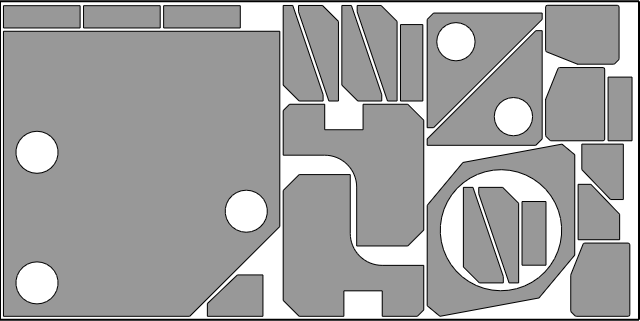
\includegraphics[width=0.9\textwidth]{nesting.png}
  \caption{Пример раскроя листа $2000 \times 1000$ мм с заданным минимальным расстоянием между деталями 10 мм}
  \label{nesting}
  \end{center}
\end{figure}

Предположим, что для вырезки деталей было использовано
$K$
сегментов резки
$S_k=M_kM^*_k; k \in \overline{1,K}$.
Тогда маршрут резки деталей можно определить
в терминах сегментов резки как кортеж

\begin{equation}
  ROUTE = (
    M_0, M_1, S_1, M_1^*, M_2, S_2, M_2^*, \dots M_K, S_K, M_K^*, i_1, i_2, \dots i_K
  )
  \label{tuple}
\end{equation}
где
$i_1, i_2, \dots i_K$
– последовательность, в которой вырезаются используемые сегменты резки
$S_1, S_2, \dots S_K$,
$M_0$
– начальная точка положения инструмента.
Линейное перемещение инструмента на холостом ходе
между точкой выключения инструмента и следующей точкой врезки
однозначно определяется этой последовательностью.
Если применить комбинаторную терминологию,
то последовательность однозначно задаётся перестановкой порядка
$K$,
т.е. упорядоченным набором натуральных чисел от $1$ до $K$
(биекцией на множестве $\overline{1,K}$),
которая числу
$k \in \overline{1,K}$
ставит в соответствие элемент
$i_k$ из набора.
Отметим, что термин «маршрут резки» является
общепринятым технологическим понятием.
В главах 3-5 при описании математических моделей оптимизации
маршрута резки мы будем использовать термин «маршрут»
применительно к перестановке
$i_1, i_2, \dots i_K$,
что, в свою очередь, соответствует устоявшейся
терминологии в задаче о последовательном обходе мегаполисов.

\begin{figure}
  \begin{center}
  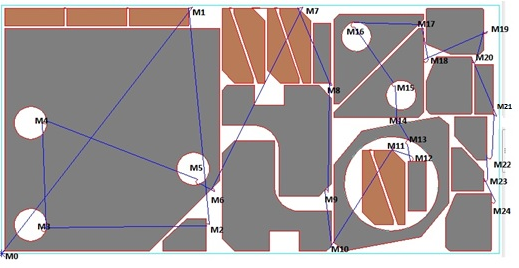
\includegraphics[width=0.9\textwidth]{cutting.png}
  \caption{Пример маршрута резки, содержащего 24 сегмента резки}
  \label{cutting}
  \end{center}
\end{figure}

На рис. \ref{cutting}
показана схема одного из возможных маршрутов резки для примера,
приведенного на Рис. \ref{nesting}.
Маршрут резки содержит 24 сегмента.
Для резки внешних контуров трёх групп деталей
с точками врезки $M_1$
(три детали в группе),
$M_7$
(четыре детали в группе) и
$M_{11}$
была использована мультиконтурная резка
(указанные группы деталей выделены коричневым цветом).
Все остальные контуры вырезаны с применением стандартной техники резки.
Последовательность резки сегментов соответствует
номерам точек врезки $M_J$ ($J=1,2,\dots 24$).
После вырезки последнего сегмента
возврат инструмента в начальную точку $M_0$
не программировался.

На приведенном рисунке визуализация траектории инструмента
осуществляется точно по граничным контурам деталей,
а не по их эквидистантным контурам, хотя,
как отмечено выше,
траектория реза должна отстоять от
граничного контура на половину ширины реза.
Это связано с тем, что в большинстве CAM – систем
программирование движения инструмента первоначально
осуществляется по граничным контурам деталей,
а вычисление реальной траектории производится
либо непосредственно самой системой ЧПУ,
либо специальной программой-постпроцессором,
предназначенной для конвертирования информации о
маршруте резки из внутреннего формата системы в
формат команд конкретного технологического оборудования с ЧПУ.
В первом случае величину припуска на рез
устанавливает оператор станке перед запуском
управляющей программы резки.

В дальнейшем без ограничения общности мы будем полагать,
что траектория инструмента в маршруте резки $ROUTE$
программируется по граничным контурам,
и сегменты резки
$S_k=M_kM^*_k; k \in \overline{1,K}$
содержат все граничные контуры деталей
$C_1, C_2, \dots C_N$,
т.е.
$$
\bigcup_{j=1}^N C_j \subset \bigcup_{k=1}^K S_k
$$
Соответственно, все точки входа в эквидистантный контур
(и выхода из эквидистантного контура)
(см. Рис. \ref{standard-cutting})
также лежат на граничных контурах.

На рис. \ref{control-program} показан фрагмент управляющей программы
(G-кода) для машины листовой газовой резки
типа «Комета» с системой ЧПУ 2Р32М.

\begin{figure}
\begin{multicols}{3}

  \%УП\_2Р32М\_01
  N1G91 \\
  N2G00X7662Y9909F6000 \\
  N3M70T1 \\
  N4M71T1 \\
  N5G01X-141Y-48F460 \\
  N6X-2400  \\
  N7X-40  \\
  N8X-67  \\
  N9X-2400  \\
  N10X-40 \\
  N11X-67 \\
  N12X-2400 \\
  N13Y-700  \\
  N14X2400  \\
  N15Y700 \\
  N16Y40  \\
  N17X107Y-40 \\
  N18Y-700  \\
  N19X2400  \\
  N20Y700 \\
  N21Y40  \\
  N22X107Y-40 \\
  N23Y-700  \\
  N24X2400  \\
  N25Y700 \\
  N26Y40  \\
  N27M74T1  \\
  N28G00X817Y-8745F6000 \\
  N29M71T1  \\
  N30G03X-108Y0I-54J0F460 \\
  N31G01Y-1048  \\
  N32X-1740 \\
  N33Y400 \\
  N34X940Y900 \\
  N35X800 \\
  N36Y-252  \\
  N37X20Y-30  \\
  … \\
  N314M71T1 \\
  N315G02X-130Y0I-65J0F460  \\
  N316G01Y267 \\
  N317G03X-50Y50I-50J0  \\
  N318G01X-1366 \\
  N319G03X-46Y-31I0J-50 \\
  N320G01X-384Y-960 \\
  N321G03X-4Y-19I46J-19 \\
  N322G01Y-1120 \\
  N323G03X14Y-35I50J0 \\
  N324G01X122Y-121  \\
  N325G03X37Y-14I35J35  \\
  N326G01X1627Y-1 \\
  N327G03X50Y50I0J50  \\
  N328G01Y1933  \\
  N329X20Y30  \\
  N330M74T1 \\
  N331M75T1 \\
  N332M02 \\
  M30
\end{multicols}
\caption{Фрагмент УП для машины листовой резки «Комета» с ЧПУ 2Р32М }
\label{control-program}
\end{figure}

Программа сгенерирована на основе маршрута резки
(спроектированного в интерактивном режиме в CAD/CAM системе «Сириус»
и показанного на Рис. \ref{cutting})
соответствующим постпроцессором со
следующими числовыми параметрами резки:
\begin{itemize}
  \item	Число строк в УП – 333;
  \item	Количество точек врезки (пробивки листа) – 24;
  \item	Путь инструмента на рабочей скорости – 27.36 метров;
  \item	Путь инструмента на быстром (холостом) ходу – 8.39 метров;
  \item	Время движения на рабочей скорости – 62.04 мин.;
  \item	Время движения на быстром (холостом) ходу – 1.64 мин.;
  \item	Общее время резки: 63.68 мин.
\end{itemize}

В зависимости от выбранного маршрута резки,
числовые параметры резки могут существенно различаться.
Таким образом, при разработке управляющих программ
для машин фигурной листовой резки с ЧПУ возникают
различные задачи оптимизации маршрута инструмента.
В качестве критерия оптимизации (целевой функции)
в этих задачах чаще всего рассматривается общее время резки.
При термической и гидроабразивной резке для сформированного
маршрута резки общее время резки
$T_{cut}$
рассчитывается по следующей формуле:
\begin{equation}
  T_{cut} = \frac{L_{on}}{V_{on}} + \frac{L_{off}}{V_{off}} +N_{pt} \cdot t_{pt}
  \label{cutting-time}
\end{equation}
где
$L_{off}$ – длина переходов с выключенным режущим инструментом (холостой ход);
$L_{on}$ – длина реза с включенным режущим инструментом;
$V_{off}$ – скорость холостого хода;
$V_{on}$ – скорость рабочего хода режущего инструмента;
$N_{pt}$ – количество точек врезки;
$t_{pt}$ – время, затрачиваемое на одну точку врезки.
При этом подразумевается,
что получаемое в результате врезки отверстие
расположено внутри материала листа.
Однако при резке заготовок, как отмечалось,
могут быть использованы и другие типы врезки,
что приводит к изменению времени врезки
$t_{pt}$
в этих случаях.
Если при резке деталей было использовано несколько типов врезки,
то формула (\ref{cutting-time}) запишется в более общем виде:
\begin{equation}
  T_{cut} = \frac{L_{on}}{V_{on}} + \frac{L_{off}}{V_{off}} +
  \sum_{j=1}^p N_{pt}^j \cdot t_{pt}^j
  \label{cutting-time-multi}
\end{equation}
где
$p$ - число использованных типов врезки,
$N_{pt}^j$ – количество точек врезки типа j;
$t_{pt}^j$ – время, затрачиваемое на одну точку врезки типа j.
И в (\ref{cutting-time}) и в (\ref{cutting-time-multi})
значение скорости холостого хода инструмента
$V_{off}$ – константа,
определяемая техническими характеристиками
используемого технологического оборудования.
Значение рабочего хода инструмента
$V_{on}$
программируется при разработке управляющей программы
в соответствии с используемой технологией резки
и параметрами листового материала
(марка материала и толщина).
Предполагается, что заданная величина
$V_{on}$  в (\ref{cutting-time}) и в (\ref{cutting-time-multi})
также является константой,
однако на практике фактическая скорость резки
может меняться в зависимости от различных технологических факторов,
а также характеристик спроектированной управляющей программы.
Это диктует необходимость проведения исследований для
определения поправочного коэффициента для величины
$V_{on}$.
В параграфе 1.4
%%% TODO ^^^^^^^^^^^^^ fix reference
будут приведены результаты такого рода исследований
применительно к машине лазерной резки с ЧПУ
ByStar 3015 для листового материала АМг3М толщиной от 1,5 до 5 мм.

Важнейшей экономической характеристикой качества
разработанной управляющей программы является стоимость
(себестоимость) резки деталей на машине с ЧПУ.
Это сложный интегрированный показатель,
который включает в себя произведённые во время
резки затраты на электроэнергию и расходные материалы,
на обслуживание машины с ЧПУ,
а также другие эксплуатационные затраты.
Отметим, что стоимость резки не всегда
пропорциональна времени резки,
поскольку зависит еще и от различных режимов резки.
По аналогии с формулой времени резки (\ref{cutting-time})
показатель стоимости резки можно определить по следующей формуле:
\begin{equation}
  F_{cost}=
  L_{on} \cdot C_{on} +
  L_{off} \cdot C_{off} +
  N_{pt} \cdot C_{pt}
  \label{cutting-cost}
\end{equation}
где
$C_{on}$ – стоимость единицы пути с включенным режущим инструментом;
$C_{off}$ – стоимость единицы пути с выключенным режущим инструментом;
$C_{pt}$ – стоимость одной точки врезки,
а $L_{on}, L_{off}, N_{pt}$
имеют тот же смысл, что и в формуле (\ref{cutting-time}).
При этом $C_{on}, C_{off}, C_{pt}$
– величины, зависящие от типа машины с ЧПУ,
технологии резки, используемой скорости рабочего хода инструмента,
толщины и марки материала.
Функциональная зависимость
$C_{on}, C_{off}, C_{pt}$
от перечисленных параметров
может задаваться либо табличными функциями,
либо аналитически.
При этом абсолютные значения этих величин
на российских предприятиях, использующих машины с ЧПУ,
определяются экономическими службами с учетом многих факторов,
и могут существенно различаться на разных предприятиях.
Зачастую стоимость резки вообще не учитывается
в раскройно-заготовительном производстве,
либо рассчитывается на основании специальных нормативов,
не зависящих от величин
$L_{on}, L_{off}, N_{pt}$.

Очевидно, что необходимость расчета стоимости резки
для каждой управляющей программы резки возникает на предприятиях,
оказывающих услуги сторонним организациям по резке материала.
Однако и на многих таких предприятиях для определения
стоимости резки учитывается только длина рабочего хода инструмента
$L_{on}$,
которая принимается равной суммарному периметру граничных контуров вырезаемых деталей
$C_1, C_2, \dots c_N$,
что, естественно, приводит к неадекватной оценке эффективности процесса резки.
В дальнейшем при оптимизации стоимостных параметров резки
мы будем применять теоретически обоснованный способ определения
показателя стоимости резки, задаваемый формулой (\ref{cutting-cost}).
На Рис. \ref{cost} представлен расчет стоимости резки
$F_{cost}$
для рассматриваемого примера при резке деталей на машине газовой резке.
Значения величин
$C_{on}, C_{off}, C_{pt}$
взяты из таблицы, используемой для расчета себестоимости фигурной
листовой резки на одном из предприятий Свердловской области.

\begin{figure}
  \begin{center}
  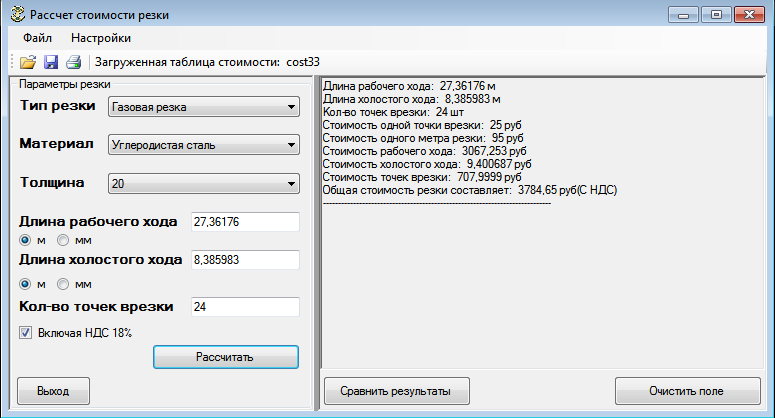
\includegraphics[width=0.9\textwidth]{cost.png}
  \caption{Пример расчета стоимости резки $F_{cost}$ при резке деталей из углеродистой стали толщины 20 мм на машине газовой резки}
  \label{cost}
  \end{center}
\end{figure}

Следует отметить,
что задача правильного определения величин
$C_{on}, C_{off}, C_{pt}$
для конкретного технологического оборудования
и конкретного материала сама по себе является малоисследованной проблемой.
В Параграфе 1.4
%%% TODO ^^^^^^^^^^^^^ fix reference
будут приведены результаты исследования,
позволяющего точно вычислять себестоимость
лазерной резки применительно для машины с ЧПУ
ByStar3015 при резке углеродистой и нержавеющей
стали различных толщин
(на примере Ст10кп и 12Х18Н10Т),
а также при резке алюминия и его сплавов (на примере Амг3М).

В случае использования нескольких типов врезки формула (\ref{cutting-cost}) примет вид:
\begin{equation}
  F_{cost}=
  L_{on} \cdot C_{on} +
  L_{off} \cdot C_{off} +
  \sum_{j=1}^p N_{pt}^j \cdot C_{pt}^j
  \label{cutting-cost-multi}
\end{equation}
где $C_{pt}^j$ - стоимость одной точки врезки типа $j$.

Как легко заметить,
значения целевых функций (\ref{cutting-time}) – (\ref{cutting-cost-multi})
однозначно определяются маршрутом резки, задаваемым кортежем (\ref{tuple}),
поскольку геометрия сегментов резки
$S_1, S_2, \dots S_K$
позволяет вычислить длину рабочего хода инструмента  $L_{on}$,
а координаты точек
$M_0, M_1, M_1^*, M_2, M_2^* \dots M_K, M_K^*$
и перестановка
$i_1, i_2, \dots i_K$
(последовательность, в которой вырезаются используемые сегменты резки),
задают набор холостых перемещений инструмента,
который определяет суммарную длину холостого хода  $L_{off}$.

Таким образом, сформулированные задачи оптимизации
маршрута инструмента для машин фигурной листовой резки с ЧПУ
можно представить в самом общем виде
как задачу минимизации некоторой числовой функции $F$,
заданной на множестве $G$ допустимых кортежей $ROUTE$, т.е.
\begin{equation}
  F(ROUTE) \to \min_{ROUTE \in G}
  \label{problem-statement}
\end{equation}

Поскольку элементы кортежа содержат
(помимо последовательности резки
$i_1, i_2, \dots i_K$,
выбираемой из дискретного множества перестановок)
точки врезки и точки выключения инструмента
$M_kM_k^*, k \in \overline{1,K}$,
которые, в свою очередь,
могут быть выбраны из континуальных подмножеств евклидовой плоскости
$\mathbb R \times \mathbb R$,
даже в случае наложения существенных ограничений
на возможность выбора допустимых сегментов
$S_k$
оптимизационная задача (\ref{problem-statement})
может быть отнесена к классу очень сложных задач
непрерывно-дискретной оптимизации.
Некоторые вопросы формирования допустимых сегментов резки мы рассмотрим в Главе 2
настоящей монографии при математической формализации задачи (\ref{problem-statement})
и ее сведении к задаче о последовательном обходе мегаполисов.
В следующем параграфе мы сформулируем основные ограничения
на допустимые значения элементов последовательности резки
$i_1, i_2, \dots i_K$
и на значения
$M_kM_k^*, k \in \overline{1,K}$,
вызванные особенностями технологии листовой резки на машинах с ЧПУ.

\subsection{Технологические ограничения на параметры маршрута инструмента машин листовой резки с ЧПУ}

\subsubsection{Ограничения на координаты точек врезки и точки выключения инструмента, обусловленные деформацией материала при врезке}

Этот тип ограничений связан с тем,
что для соблюдения технологии врезки любая точка врезки
$M_k$
должна лежать (как отмечалось выше)
на некотором ненулевом расстоянии от контура детали,
по которому движется инструмент.
При этом координаты точки врезки должны,
естественно, находиться вне областей,
занимаемых геометрическими образами других деталей с учетом припуска на рез.
Величины необходимых минимально допустимых расстояний
от контуров детали до точек врезки и точек выключения
инструмента определяются различными технологическими параметрами.
Другими словами, этот тип ограничений носит геометрический характер
и определяет геометрические области на раскройной карте,
в которых допустимо задавать точки врезки для формирования сегментов резки.

Для общей формализации этих ограничений обозначим через
$E_j^d$ – эквидистанты замкнутых контуров $C_j$,
удаленные от них на величину $d$,
а через
$P_j^d$ – двумерные геометрические объекты (замкнутые точечные множества),
ограниченные этими эквидистантами
$P_j^d \subset E_j^d \subset \mathbb R^2$.
При этом будем полагать,
что для внешних контуров деталей  является внешней эквидистантой,
а для внутренних – внутренней.
Пусть $ОUT$ - конечное множество индексов внешних контуров деталей,
а $IN$ – соответственно множество индексов внутренних контуров.
Обозначим  размерность этих множеств соответственно $l$ и $s$,
т.е.
$OUT = \{j_1, j_2, \dots j_l\};
IN = \{q_1, q_2, \dots q_s\}$
$(OUT  \subseteq \overline{1,N};
(OUT  \subseteq \overline{1,N})$.
Заметим, что если $l=N$
(все контуры являются внешними), то
$IN = \varnothing$.
Пусть $d1$ – минимально допустимое расстояние от контуров деталей до точек врезки,
тогда выбранные точки врезки для каждого сегмента резки должны удовлетворять следующим условиям:
\begin{equation}
  \forall k \in \overline{1,K}:
  M_k \in G_M;
  G_M = \big(B \setminus \bigcup_{j\in OUT} P_j^{d1} \big) \bigcup_{q\in IN}P_q^{d1}
  \label{pierce-constraint}
\end{equation}

Как мы уже отмечали,
минимально допустимое расстояние от граничных контуров деталей
до точек врезки,
задаваемых на границе листа,
или подготовленных предварительно механическим способом,
может быть несколько меньше,
чем до точек врезки, получаемым стандартным «прожиганием» (пробивкой) материала листа.
Для таких особых точек врезки область $G_M$,
задаваемая условием (\ref{pierce-constraint}),
может быть расширена.
Это условие являются необходимым, но не достаточным,
и для конкретных задач могут возникать дополнительные ограничения,
обусловленные технологическими особенностями резки,
о которых пойдёт речь ниже.
В этих случаях, наоборот, область $G_M$
может быть существенно сокращена.

Аналогичное условию (\ref{pierce-constraint})
ограничение справедливо и для точек выключения инструмента:
\begin{equation}
  \forall k \in \overline{1,K}:
  M_k^* \in G_{M^*};
  G_{M^*} = \big(B \setminus \bigcup_{j\in OUT} P_j^{d2} \big) \bigcup_{q\in IN}P_q^{d2}
  \label{tool-off-constraint}
\end{equation}
где $d2$ – минимально допустимое расстояние
от контуров деталей до точек выключения инструмента,
которое, чаще всего, меньше $d1$
и может, как отмечалось, быть и нулевым.

На Рис. \ref{pierce-area} красным цветом показаны геометрические области листа,
допустимые для определения точек врезки при программировании резки
внешних граничных контуров деталей,
обозначенных на рисунке 1,2 и 3 и внутреннего граничного контура 4.
При этом минимально допустимое расстояние $d1$ от граничных контуров 1-4 до возможных точек врезки,
установленное пользователем CAM – системы, равно 9,5 мм.

\begin{figure}
  \begin{center}
  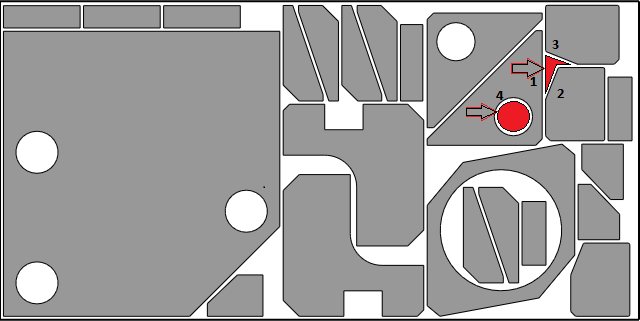
\includegraphics[width=0.9\textwidth]{pierce-area.png}
  \caption{Пример двух геометрических областей на раскройной карте (выделены красным цветом), допустимых для задания точек врезки }
  \label{pierce-area}
  \end{center}
\end{figure}

\subsubsection{Условие предшествования}

Это условие накладывает ограничения на порядок вырезки сегментов
$ I = (i_1, i_2, \dots i_K)$.
Ограничения на порядок их резки обусловлены особенностями
технологии и оборудования листовой резки с ЧПУ,
которые не позволяют после вырезки внешнего контура точно
позиционировать инструмент для вырезки внутренних контуров,
поскольку деталь после вырезки внешнего контура может
изменить свое положение на раскройном столе.
Это вызвано тем, что после вырезки внешнего контура
вырезанная деталь «теряет» связь с листом,
а для многих типов раскройных столов эта деталь
может даже изменить свое положение относительно плоскости листа
(упасть между статическими конструкциями раскройного стола).
При выборе последовательности контуров следует придерживаться следующих правил.

{\it Правило 1}.
Если внешний контур имеет один или более внутренних контуров,
которые представляют собой границы отверстий в деталях,
то прежде, чем будет начата вырезка внешнего контура,
должны быть вырезаны все внутренние контуры.

{\it Правило 2}.
Если внутренний контур детали на раскройной карте
содержит внешний контур/контуры другой детали,
то сначала должна быть вырезана эта другая деталь
с соблюдением {\it Правила 1}.

Перечисленные правила и называются условием предшествования для перестановки
$ I = (i_1, i_2, \dots i_K)$.
В терминах её элементов условие означает следующее:
\begin{enumerate}
  \item
  если в перестановке
  $ I = (i_1, i_2, \dots i_K)$
  сегмент $i_k$
  содержит внешний контур,
  то все соответствующие внутренние контуры должны содержаться в сегментах,
  предшествующих сегменту $i_k$
  в перестановке;
  \item
  если в перестановке
  $ I = (i_1, i_2, \dots i_K)$
  сегмент $i_k$
  содержит  внутренний контур,
  который на раскройной карте содержит внутри внешний контур,
  соответствующий другому объекту
  $A_l$
  $(l=1,2, \dots n)$,
  то этот внешний контур должен быть вырезан в сегментах,
  предшествующих сегменту $i_k$ в перестановке $I$.
\end{enumerate}

Рис. \ref{precedence} иллюстрирует условие предшествования
при формировании маршрута резки для деталей,
содержащих внутренние контуры.

\begin{figure}
  \begin{center}
  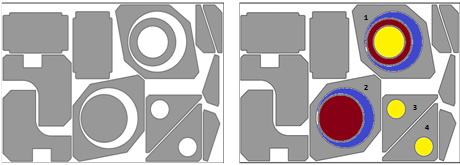
\includegraphics[width=0.9\textwidth]{precedence.png}
  \caption{Пример раскройной карты деталей, содержащих внутренние контуры}
  \label{precedence}
  \end{center}
\end{figure}

В соответствии с условиями предшествования резка контуров,
ограничивающих цветные области для 4-х деталей на Рис. \ref{precedence},
должна осуществляться в следующей последовательности:

\begin{enumerate}
  \item жёлтый, красный, синий, серый;
  \item	красный, синий, серый;
  \item	жёлтый, серый;
  \item жёлтый, серый.
\end{enumerate}

Условия предшествования и ограничения на координаты точек врезки
и точки выключения инструмента,
обусловленные деформацией материала при врезке,
имеют статический характер,
т.е. однозначно определяются спроектированной раскройной картой,
используемым для резки технологическим оборудованием
и свойством раскраиваемого материала.
В терминах маршрута резки $ROUTE$
и его параметров
$M_0, M_1, S_1, M_1^*, M_2, S_2, M_2^*, \dots M_K, S_K, M_K^*,$
$i_1, i_2, \dots i_K$
технологическое ограничение
1) однозначно определяет допустимые геометрические области
$G_M$
и
$G_{M^*}$
для выбора точек врезки и точек выключения инструмента,
а технологическое ограничение
2) накладывает запрет на некоторые значения перестановки
$ I = (i_1, i_2, \dots i_K)$
при формировании порядка резки сегментов. При
этом сформулированные требования не зависят от задаваемых параметров кортежа
$ROUTE$.

В отличие от этих двух технологических ограничений
следующий тип технологических требований устанавливает
дополнительные ограничения на выбор точки врезки и выбор
порядка резки сегментов на каждом шаге формирования маршрута резки
(т.е. при определении параметров очередного выбираемого сегмента)
в зависимости от того какие параметры маршрута резки были выбраны на предыдущих шагах.
Этот тип ограничений обусловлен геометрическими
искажениями материала при термической резке деталей.

\subsubsection{Эвристические правила термической резки заготовок из листовых материалов}

Термические воздействия на вырезаемые заготовки можно подразделить на два типа\footnote{
  Сформулированные в п.3)
  правила разработаны сотрудниками ОАО «Уралхиммаш»
  В.И.Кротовым и А.Д.Гуртовенко на основе опыта
  резки листовых материалов на машинах термической резки с ЧПУ
  в котельно-заготовительном комплексе предприятия в 1992г
}:

\begin{itemize}
\item общие изменения геометрических размеров заготовки (уменьшение)
вследствие ее вырезания из нагретой части материала;
\item	изменение геометрической формы заготовок
(изменение радиусов у секторов,
отклонения от прямолинейности у прямоугольных деталей) и др.
Чем больше геометрические размеры заготовки,
тем больше изменения.
Наиболее  подвержены данным изменениям узкие длинные заготовки.
\end{itemize}

В Таблице \ref{thermal-classification}
приведена типология некоторых видов заготовок
по признаку подверженности термическим деформациям.
В качестве основных геометрических характеристик
классификации заготовок использованы габаритные размеры заготовок
(A - габаритная длина, B - габаритная ширина).
Приведенные в таблице типы заготовок относятся,
в основном, к номенклатуре машиностроительных предприятий,
но широко используются также в раскройно-заготовительном производстве
других отраслей промышленности.

\begin{table}
  \begin{tabular}{ p{0.3\textwidth} p{0.3\textwidth} p{0.3\textwidth} }
  Термическая характеристика заготовки
    & Описание заготовки
    & Геометрические характеристики заготовки \\
  \hline
  Заготовки, подверженные термическим деформациям изгиба
    & Полосы, узкие обечайки, секторы
    &	$B<100 \text{мм}, A>5B$ $100<B<250, A>8B$ \\
  Заготовки, подверженные термическим деформациям изгиба и изменением длины
    & Длинномерные и узкие полосы и обечайки, длинномерные секторы больших радиусов ($R>200$ мм)
    & $B <100 \text{мм}, A>10B$ $100<B< 300, A>15B$ \\
  Заготовки, не подверженные термическим деформациям
    & Фланцы, заглушки, диски, косынки, ребра, стенки, широкие сегменты и обечайки
    & $A/B < 5$ \\
  Заготовки, подверженные оплавлению и загрязнению при резке
    & Малогабаритные косынки, планки, ребра
    & $ A, B <200 \text{мм}$ \\
  Заготовки, вырезаемые с большим удельным тепловыделением
    & Полосы, обечайки, секторы со скосами кромок под сварку
    & $ A>300 \text{мм}, B>150 \text{мм}$ \\
  \hline
  \end{tabular}
  \label{thermal-classification}
  \caption{Классификация заготовок по признаку подверженности термических деформаций}
\end{table}

В зависимости от термических характеристик заготовок
и от требований к их точности выбирается оборудование,
способ и последовательность резки.
Например, величина удельного тепловыделения –
наибольшая при газокислородной резке,
поэтому имеет смысл тонкие листы из углеродистых и
низколегированных сталей резать плазменно-дуговым способом,
дающим попутно большой выигрыш в производительности.
Металлы, обладающие более высокой теплопроводностью
менее склонны к термическим деформациям.
Термообработка листового проката уменьшает
тепловые деформации материала и наоборот:
необработанный лист более склонен к термическим деформациям,
т.к. в нем присутствуют высокие внутренние  напряжения,
которые накладываются на усилия, возникающие от  нагрева при резке.

На величину термических деформаций оказывают влияние:
\begin{itemize}
\item	тип резки (газовая, плазменная, лазерная);
\item	марка материала (его теплопроводность);
\item	состояние поставки металла (наличие внутренних напряжений), его термообработка;
\item	толщина металла;
\item	выбор порядка резки заготовок;
\item	выбор точек врезки для каждого контура;
\item	направление обхода контура (по/против часовой стрелки).
\end{itemize}

При работе в интерактивном режиме в CAM системе
пользователь может сам определять контуры или их части
для формирования сегментов резки,
выбирать порядок резки сегментов и координаты точек врезки
в нужном месте посредством курсора «мыши».
Автоматический режим предполагает наличие в CAM системе
соответствующего алгоритма определения маршрута резки $ROUTE$
с соблюдением необходимых технологических требований.
Сформулируем наиболее важные из технологических требований резки,
обусловленные наличием термических деформаций материала.
Прежде всего, введем понятия правил «жесткости заготовки» и «жесткости материала».

\paragraph{Правило «жесткости заготовки» («жесткости детали»)}

Правило «жесткости заготовки/детали» касается выбора точек врезки
$M_k, k \in \overline{1,K}$
в маршруте резки  $ROUTE$,
а также выбора направления резки контуров деталей.
Оно заключается в том, что при резке контура точка
врезки и направление резки контура выбираются таким образом,
чтобы сначала вырезались участки контура,
расположенные в непосредственной близости к границе материала,
либо к границе вырезанной области,
а завершение резки происходило по участку контура,
граничащего с «жесткой» (не вырезанной) частью области.

Поясним правило «жесткости заготовки» на примере.
На Рис. \ref{part-hardness}
показаны 3 заготовки и 9 выбранных возможных точек врезки.

Предположим, что мы начинаем резку с заготовки «А»
и выбираем одну из первых 4 точек врезки (1-4).
Точка 2 является недопустимой для врезки,
поскольку при завершении резки не остается
«жесткого» участка не вырезанной области в материале,
и заготовка (еще до завершения резки контура)
начнет перемещаться относительно материала.
Кроме этого, заготовка будет получать максимальное
нагревание из-за малой площади остатка в области завершения резки.
Все это, в конечном итоге,
приведет к искажению геометрических размеров заготовки.

\begin{figure}
  \begin{center}
  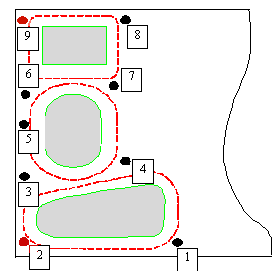
\includegraphics[width=0.5\textwidth]{part-hardness.png}
  \caption{Пример выбора точек врезки}
  \label{part-hardness}
  \end{center}
\end{figure}

Точки 1,3 и 4 являются допустимыми для врезки,
однако при выборе точки врезки 1 резка контура
должна производиться по часовой стрелке,
а при выборе точки 3 - против.
Для точки 4 – направление реза не является существенным.
При резке следующей заготовки («Б»)
допустимы точки врезки 4,6 или 7.
Для точки 4 правило «жесткости заготовки»
предполагает движение резака по часовой стрелке,
а для точки 6 – против часовой стрелки.

И, наконец, при резке заготовки «В»
допустимы точки врезки 7 или 8.
Выбор точки врезки 7 диктует необходимость
движения резака по часовой стрелке,
а в случае выбора точки 8 – против часовой стрелки.

Таким образом, правило «жесткости заготовок»
существенно ограничивает свободу выбора точек
врезки и направлений обхода контура.
В частности, для данного примера,
если все контуры вырезаются по часовой стрелке,
то набор точек врезки 1, 4, 7
является наиболее предпочтительным,
а если – против часовой стрелки, то – 4, 7, 8
(или 4,6,8).
Понятно, что строгая формализация процедуры
выбора представляется затруднительной,
и остальные допустимые варианты также не приведут
к критическим изменениям в геометрии заготовок,
но интуитивно ясно, что предлагаемые 3 варианта
несколько уменьшат тепловые деформации по сравнению
с другими допустимыми вариантами.

Важно отметить,
что при изменении порядка вырезки заготовок
(например, в последовательности «В», «Б», «А»)
изменится и набор допустимых точек врезки и направлений реза.

Функция определения допустимых
(как с точки зрения геометрических характеристик,
так и с точки зрения технологических требований резки)
точек врезки является важнейшей функцией CAM – системы
при автоматическом режиме формирования УП.

\paragraph{Правило «жесткости материала» («жесткости листа»)}

Это правило определяет допустимый порядок
(последовательность)
$i_1, i_2, \dots i_k$,
в которой вырезаются используемые сегменты резки
$S_1, S_2, \dots S_K$.
Фактически это правило включает в себя несколько эвристических правил.
Рис. \ref{list-hardness}
иллюстрирует 4 правила выбора стороны материала,
с которой следует начинать процесс термической резки.
Правило а) рекомендует начинать процесс резки с узкой стороны листа (материала).
Правила б), в) и г) уточняют,
какую из узких сторон выбрать.
Алгоритм выбора заключается в следующем.

\begin{enumerate}
  \item
  Сначала определяем,
  есть ли среди заготовок длинномерные детали
  (длинномерной деталью в соответствии с Таблицей \ref{thermal-classification}
  будем называть заготовки, у которых один из габаритов больше другого не менее,
  чем в 10 раз).
  Если эти заготовки расположены вблизи
  узкой границы материала,
  то процесс резки следует начинать с них
  (правило б),
  так как именно такого рода заготовки
  подвержены максимальным тепловым деформациям.
  \item
  Затем определяем,
  есть ли на материале крупный отход.
  При наличии такого отхода с одной из сторон,
  процесс резки следует начать с противоположной стороны,поскольку аккумулирующееся в материале в процессе резки
  тепло в конечной стадии резки должно быть
  несколько скомпенсировано «жестким» остатком
  (правило в).
  \item
  И, наконец,
  если на материале нет крупного отхода,
  резку следует начинать с той стороны,
  где суммарные тепловыделения от резки больше
  (больше мелких деталей, либо больше суммарный периметр реза)
  (правило г).
\end{enumerate}

\begin{figure}
  \begin{center}
  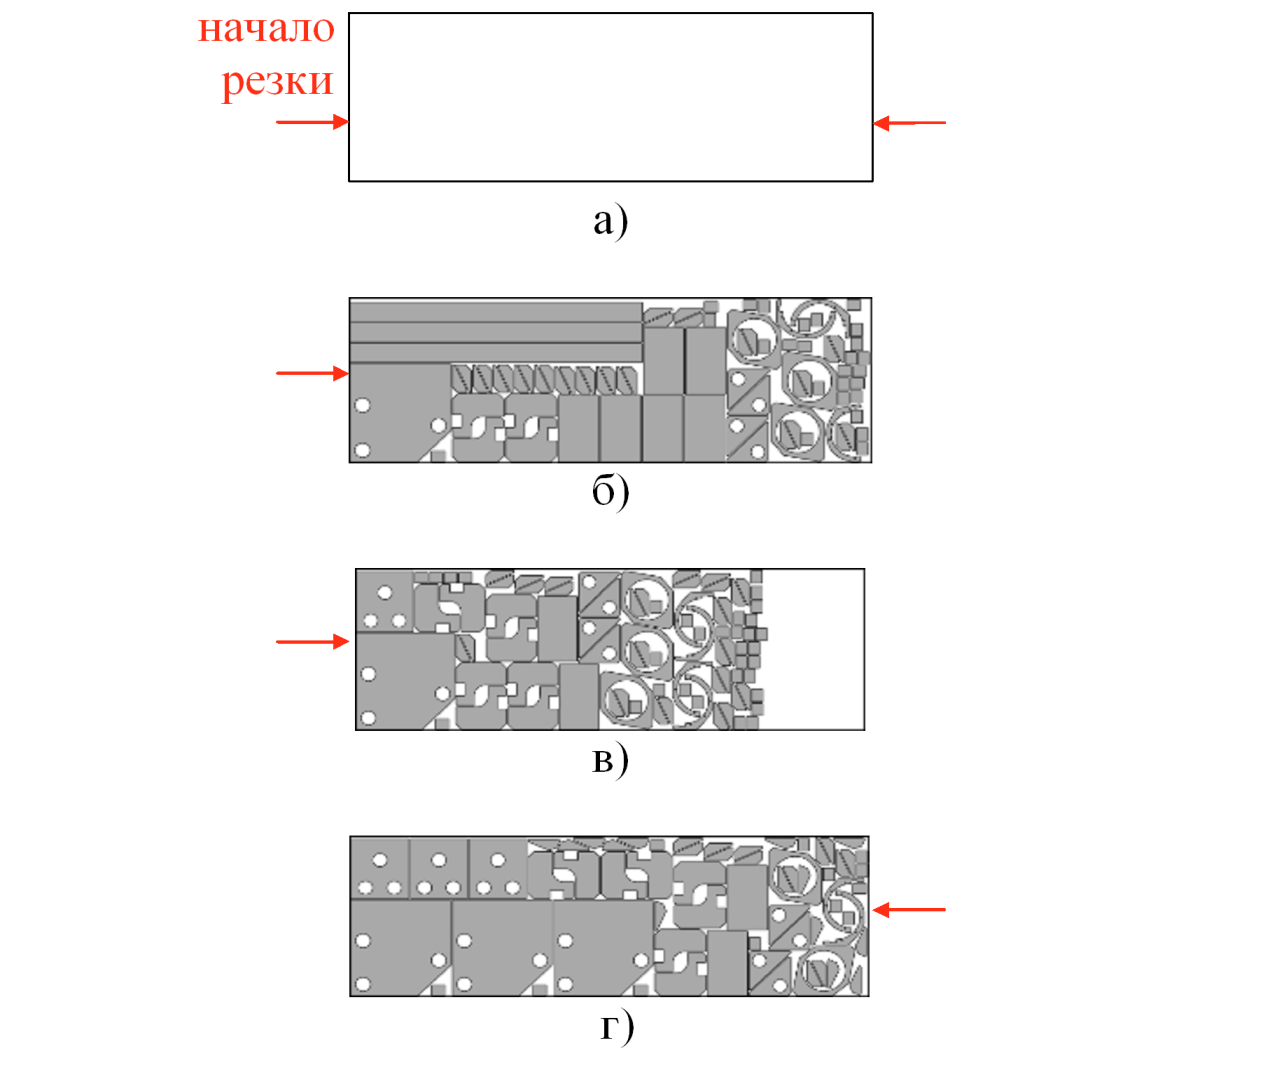
\includegraphics[width=0.9\textwidth]{list-hardness.png}
  \caption{Правила выбора начальной стороны материала }
  \label{list-hardness}
  \end{center}
\end{figure}

Еще два правила «жесткости» заключаются в том,
что при выборе последовательности вырезаемых заготовок
на материале не должно оставаться узких полос и «островов»,
содержащих не вырезанные заготовки
(см. Рис. \ref{island}).

\begin{figure}
  \begin{center}
  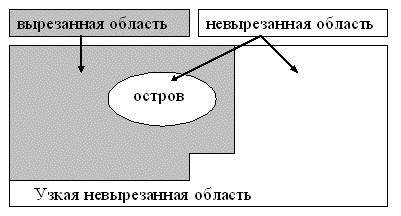
\includegraphics[width=0.6\textwidth]{island.png}
  \caption{Пример материала с недопустимыми не вырезанными областями}
  \label{island}
  \end{center}
\end{figure}

Для того чтобы обеспечить все правила «жесткости материала»,
следует предварительно разбить всю область резки на некоторые «зоны»
и затем процесс резки заготовок осуществлять
в этих зонах последовательно по возрастанию номеров зон,
т.е. область размещения $В$ разбивается на подобласти
\begin{equation}
  B_j = \bigcup_{r=1}^l \Omega_r
\end{equation}

где $l$
– количество выбранных зон для области $B$.
При этом формирование и нумерация зон
должна проводиться в соответствии со всеми правилами
«жесткости материала» и таким образом,
чтобы оставшаяся не вырезанная область
по своей геометрической форме приближалась к квадратной области.

Пример разбиения области термической резки на зоны
представлен на
Рис. \ref{zones}.
Зона 1 и зона 8,
выделенные на рисунке темно-серым цветом,
сформированы с учетом правила «жесткости материала» б).

\begin{figure}
  \begin{center}
  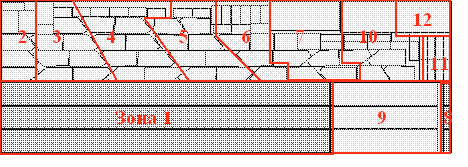
\includegraphics[width=0.9\textwidth]{zones.png}
  \caption{Пример формирования зон резки с учетом «жесткости» материала}
  \label{zones}
  \end{center}
\end{figure}

\paragraph{Заключительные замечания}

В настоящее время в научных публикациях по теме настоящей монографии
наименее изученными остаются вопросы математической формализации ограничений,
связанных именно с технологическими требованиями термической резки.
Следует отметить, что правила «жесткости заготовки» и «жёсткости материала»
целесообразно учитывать (как показала практика)
не только при разработке управляющих программ для машин газовой,
плазменной и лазерной резки с ЧПУ,
но и при применении машин гидроабразивной фигурной листовой резки.
Этот факт свидетельствует о том,
что изменения геометрических характеристик материала
связано не только с термическими деформациями,
но и с механическими трансформациями материала
при листовой резке заготовок на машинах с ЧПУ.
Рекламные заявления некоторых производителей
лазерных и гидроабразивных машин с ЧПУ о незначительных
деформациях вырезаемых заготовок при листовой фигурной
резке на данных типах технологического оборудования с ЧПУ
опровергаются практическими исследованиями.
Разумеется, лазерная и гидроабразивная технологии
порождают меньшие проблемы с тепловыми деформациями материала,
чем газовая и плазменная,
но не исключают полностью геометрические искажения формы заготовок при резке.

Если обозначить через
$ROUTE_\nu$
частичный маршрут резки первых $\nu$
сегментов
$\nu < K$
\begin{equation}
  ROUTE_\nu = (M_0, M_1, S_1, M_1^*, \dots M_\nu, S_\nu, M_\nu^*, i_1, i_2, \dots i_\nu)
\end{equation}

то правила «жесткости заготовки» и «жёсткости материала»
при формировании допустимого маршрута
$ROUTE$
помимо соблюдения условий предшествования для перестановки
$i_1, i_2, \dots i_K$
и условий (\ref{pierce-constraint}) и (\ref{tool-off-constraint})
формирует следующее дополнительное условие:
если
$ROUTE_\nu$ - частичный маршрут,
допустимый с точки зрения всех технологических
требований листовой резки 1)-3),
сформулированных в этом параграфе,
то сегмент с номером $\nu+1$
и соответствующая точка врезки $M_{\nu+1}$
для него в маршруте
$ROUTE_{\nu+1}$
должны выбираться с учетом уже выбранного частичного маршрута
$ROUTE_\nu$,
что фактически означает либо запрет
на некоторые «плохие» номера сегментов
$i_{\nu+1}$
и «плохие» точки врезки
$M_{\nu+1}$
в области  $G_M$,
либо наложение «штрафа» на «плохие» значения
этих параметров кортежа
посредством включения наложенного штрафа в целевые функции
(\ref{cutting-time}) – (\ref{cutting-cost-multi})
при решении оптимизационной задачи (\ref{problem-statement}).

Таким образом,
условия «жесткости заготовки» и «жёсткости материала»
порождают для задачи непрерывно-дискретной оптимизации (\ref{problem-statement})
своего рода динамические ограничения,
формируемые только в процессе вычисления допустимого решения задачи.
В параграфе 2.1
%%% TODO ^^^^^^^^^^^^^^^ fix reference
настоящей монографии будут изложены
некоторые способы математической формализации динамических ограничений,
и описаны алгоритмы оптимизации,
учитывающие эти ограничения.

\paragraph{Классификация оптимизационных задач маршрутизации инструмента машин фигурной листовой резки с ЧПУ}

\end{document}
